\documentclass[11pt]{article}
\usepackage{a4wide}
\usepackage{float}
\usepackage{graphicx}
\usepackage{hyperref}
\usepackage[margin=1in,footskip=0.25in]{geometry}
\graphicspath{{./images/}}

\begin{document}

\begin{titlepage}
\title{Reinforcement learning gebaseerde agent voor presidenten}
\author{Freya Van Speybroek \& Thor Dossche}
\date{Academiejaar 2020 \- 2021}
\maketitle
\thispagestyle{empty}
\end{titlepage}


\section{Inleiding}
In dit project zullen we bestuderen hoe reinforcement learning kan toegepast worden op een kaartspel. Het kaartspel dat we gaan bekijken is presidenten. Dit is een perfect voorbeeld van een spel waarbij we incomplete informatie hebben: er kan namelijk niet in de kaarten van de tegenstanders gekeken worden. Daarbij is elke toestand discreet, waardoor het probleem kan gemodelleerd worden als een Partially Observable Markov Decision Process (POMDP).\\\\
Voor dit soort problemen zijn er al heel wat oplossingsmethodes, waarvan we er een paar zullen uitproberen en vergelijken. Daarbij kunnen we ons ook de vraag stellen of het wel degelijk rendeert om Reinforcement Learning te gebruiken, misschien zijn we beter af met een heuristiek? 

\subsection{Het probleem}
Presidenten kent veel varianten, de regels liggen namelijk niet hard vast en kunnen daarom vaak besproken worden onder de spelers. Afhankelijk van welke regels je gebruikt, kan het spel moeilijker worden. \\\\
Bij het spelen van presidenten speel je meerdere spelletjes. Na ieder spel zullen de `rangen' voor het volgend spel gekend zijn. Ieder spel bestaat uit meerdere rondes. In deze rondes proberen de spelers zoveel mogelijk kaarten te leggen om zo al hun kaarten uit te spelen. Tijdens een ronde moeten spelers elk om beurt een kaart leggen hoger of gelijk aan de vorige kaart. Het aantal van die kaarten moet hoger of gelijk zijn aan de kaart(en) van de vorige beurt.\\
Als een speler geen kaart(en) meer kan of wil liggen past hij, eenmaal gepast zal hij niet meer aan de beurt komen in de ronde. Als alle spelers op een na gepast hebben is de winnaar van de ronde gekend. Deze speler mag een nieuwe ronde starten met een kaart of kaarten naar keuze. Als een speler al zijn kaarten heeft uitgespeeld krijgt hij een rang toegewezen voor het volgende spel.\\
De persoon die het eerste uitspeelt is de president, de tweede de vice-president.
De persoon die als laatste overblijft is de scum, degene die als voorlaatste uitspeelt is de vice-scum.\\
Als alle rangen gekend zijn start het volgende spel. Na het delen van de kaarten krijgt de president de beste 2 kaarten van de scum, de scum krijgt de 2 slechtste van de president. Hetzelfde geldt voor vice-president en vice-scum, maar die wisselen slechts 1 kaart uit.\\\\
Nog enkele basisregels:\\\\
- De speler die de ‘klaver 3’ heeft, start de eerste ronde van een spel met deze kaart (of meerdere kaarten van waarde 3 waaronder de `klaver 3'). \\
- Als een speler uit is, dan wordt een nieuwe ronde gestart en mag de speler links van de net uitgespeelde speler beginnen.\\\\
Om het spel interessanter te maken hebben wij nog een paar extra regels toegevoegd:\\\\
- Als een 7 is gespeeld, dan moet de volgende kaart lager of gelijk zijn aan die 7 ook het aantal kaarten moet gelijk zijn aan het aantal gelegde kaarten.\\
- De kaart 2 is een joker die kan gebruikt worden als hoogste kaart in het spel, of als een extra kaart. Als de joker gelegd wordt samen met een kaart van een andere waarde zal de joker deze waarde aannemen.\\
- De ranking van de kaarten is dus als volgt: 3,4,5,6,7,8,9,10,V,Q,K,A,2\\

\subsection{De environment}
Bij Reinforcement Learning gaan we niet aan de slag met een dataset, maar met een “environment”, die het spel zelf voorstelt. We willen dan een agent bekomen die een zo hoog mogelijke score behaalt in de environment. \\
In dit geval, willen we een agent die zo vaak mogelijk of zo lang mogelijk president kan zijn. Maar, de situatie is niet zo zwart-wit. Het is namelijk ook goed zijn om veel vice-president te zijn want dan ben je nog steeds in een voordeelpositie. Goed spelen kan ook zijn dat je met zeer slechte kaarten toch niet scum wordt maar door tactisch te spelen de high-scum rang behaalt. Soms krijg je gewoon kaarten waarmee je gewoon niet kan winnen hoe goed je ook bent, heb je dan slecht gespeeld als je scum wordt? Het is duidelijk niet zo dat dat altijd winnen een goeie maat is om te meten of je goed bent. Er zal dus gezocht moeten worden naar een goed evenwicht van deze verschillende factoren om te bepalen of de agent goed is. \\
Bovendien kan de environment ook op veel verschillende manieren bekeken worden. Hoe wordt een state voorgesteld, welke rewards delen we uit, welke acties maken we mogelijk? Dit zijn allemaal deelproblemen op zich, waarvoor we verschillende oplossingen zullen proberen vinden.\\\\

\subsection{Mogelijke oplossingsmethoden}
Zoals in de inleiding besproken, is ons probleem gemodelleerd als  een Partially Observable Markov Decision Process (POMDP). Hier zijn verschillende oplossingsmethoden voor mogelijk, waaronder Q-learning, DQN en Monte Carlo Tree Search. Het doel van deze oplossingsmethoden en van Reinforcement Learning zelf, is om een agent, gegeven een toestand en een aantal acties, de meest optimale actie te laten kiezen. Hierbij wordt met optimaal bedoeld dat de agent zijn score maximaliseert. Een actie uitvoeren in een bepaalde state, geeft de agent dus een reward (die goed of slecht kan zijn).\\\\ 
Een eerste interessante weg is Q-learning. Alhoewel dit een algoritme is dat we vaak bij simpele spelsituaties gebruikt zien (zoals \cite{simple-qlearning}), zouden we kunnen kijken of dit goede resultaten geeft. Aangezien Q-learning werkt met een Q-table die per state en per actie een score bijhoudt, kan het toch zijn dat dit te beperkt is voor de grote aantal mogelijke spelsituaties in presidenten. \\\\
Het is daarom misschien interessanter om met een DQN of Deep Q-Network te werken, waarmee we kunnen werken met grotere states om zo meer informatie over het spel bij te houden. Een succesvol voorbeeld met neurale netwerken is \cite{nn-paper}, waar ze werken met spel dat een gelijkaardige complexiteit heeft als presidenten. Waarom ze niet met DQN werken, wordt ook besproken, en is interessant om later in dit onderzoek nog eens aan te halen. \\\\
Ten laatste zou Monte Carlo Tree Search een zelfde beperkingen geven als Q-learning, namelijk de grootte van de state. Hoe groot kunnen we de state maken tot we in een situatie komen waar we te veel paden hebben om te simuleren? Hiervoor zijn er wel al oplossingen, waaronder Partially Observable Monte-Carlo Planning (POMCP), wat een aangepaste Monte Carlo tree search is om POMDPs op te lossen \cite{mct-1}. Er bestaan ook andere manieren door Monte Carlo te combineren met andere oplossingen, zoals in \cite{mct-2} of \cite{mct-3}.\\\\

\section{Methodiek}
Uit de bovenstaande besproken oplossingsmethodes, bespreken we de eerste twee, namelijk Q-learning en DQN. Interessant hieraan is dat de tweede methode, die met een Deep Q-Network werkt, gebaseerd is op het Q-learning van de eerste methode. Ook bekijken we een alternatieve, eenvoudigere oplossingsmethode die aan de hand van heuristieken of vuistregels van presidenten werkt.\\

\subsection{Heuristiek}

Om te toetsen hoe goed de andere oplossingsmethoden zijn, hebben we een goede speler nodig. Hiervoor hebben we een heuristiek geimplementeerd die ongeveer volgt wat echte spelers in het spel zouden doen, namelijk:\\
\begin{itemize}
	\item Leg altijd de laagste kaart mogelijk. Als je meerdere van die kaart hebt, leg ze allemaal.
	\item Leg enkel een joker als je niet anders kan.
	\item Pas enkel wanneer je niets kan leggen.
\end{itemize}
Een echte speler zal natuurlijk ook rekening houden met details zoals welke kaarten al gelegd zijn doorheen het spel, hoeveel spelers al uitgespeeld zijn, ... Maar we zullen toch zien dat deze heuristiek opvallend goede resultaten behaald. \\\\
Ook hebben we een extra speler geimplementeerd: de random speler. Deze speler kiest een willekeurige zet uit de mogelijke zetten die hij op dat moment kan doen gegeven de laatst gelegde kaart(en) en de kaarten in zijn hand. Zo hebben we nu een goede en slechtere speler, waarop getest kan worden.\\\\

\subsection{Q-learning}
\subsubsection{Theorie}
Q-learning helpt ons zoeken naar een zo goed mogelijke policy \textbf{(todo: leg policy uit? zie dqn-pract)}. De letter $Q$ slaat op de functie die gebruikt wordt om, gegeven een state en een actie, de waarde van deze combinatie te vinden. Deze waarde geeft aan hoe goed - of slecht - een bepaalde actie is in een bepaalde state.\\\\
Op basis van de Bellman equations \cite{bellman-equations}, kunnen we een update regel definieren die er als onderstaande formule uitziet. Een Q-waarde van een bepaald state-actie paar zal dus veranderen met de tijd. Daarom moeten we in het begin de Q-waarden initialiseren, om die dan wanneer nodig aan te passen.\\\\


\begin{figure}[h]
\centering
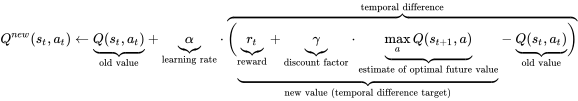
\includegraphics[scale=0.70]{images/qformula.png}
\caption{Q function - Source: wikipedia.org/wiki/Q-learning}
\end{figure}

Er zijn nog een aantal belangrijke parameters aanwezig in de formule. 
\begin{itemize}
	\item Learning rate: Geeft aan in welke mate we de Q-waarde updaten, een grote learning rate zal dus meer impact hebben op de uiteindelijke Q-waarde dan een kleinere.
	\item Reward: Score die berekend wordt op basis van de state waar we in waren en de gekozen actie. Door deze actie uit te voeren, komen we in een nieuwe state en kunnen we kijken hoe waardevol deze actie was. 
	\item Discount factor: Geeft aan hoe belangrijk toekomstige rewards zijn. Een hoge discount factor zal meer belang hechten aan rewards over een lange tijd, een lage discount factor laat het algoritme enkel rewards in een korte tijdsperiode beschouwen.
	\item Estimate of optimal future value: In deze stap gaan we de Q-waarden overlopen over alle mogelijke acties in de volgende state, en halen we de hoogste Q-waarde eruit. Merk op dat als de discount factor 0 is, dit niet uitmaakt, en dus niet naar toekomstige states of rewards kijken.
\end{itemize}

Daarbij is het in Q-learning belangrijk om te beschouwen hoe we de volgende actie a kiezen, om dan overeenkomende $Q(s,a)$ aan te passen. We zouden elke keer de beste actie kunnen kiezen op basis van de Q-waardem, maar dit zal in begin niet werken, aangezien er dan nog helemaal niets geleerd is. We willen dus genoeg exploratie hebben, zeker in het begin! Een oplossing hiervoor is om een $\epsilon$-greedy policy te volgen. Waarbij we met kans $\epsilon$ een willekeurige actie kiezen, en met kans $1-\epsilon$ een actie kiezen gebaseerd op de huidige policy. We kunnen deze $\epsilon$ eventueel laten variëren met de tijd.\\

\subsubsection{Implementatie}
De Q-waarden die doorheen het algoritme geupdate worden, worden bijgehouden in een Q-table. In onze eerste implementatie houdt de state 2 velden bij die de laatst gelegde kaart en zijn hoeveelheid voorstellen. De state wordt gegeven als een tuple (rang, aantal), en acties worden op dezelfde manier voorgesteld. Zo indexeren we de Q-table met deze 2 tuples. \\\\
We kunnen natuurlijk bediscussiëren of het niet beter zou zijn om een grotere state bij te houden, maar hier komen we later bij onze testresultaten op terug. Er is wel een beperking in hoe groot we de state kunnen maken, aangezien er een punt zou zijn waar de tabel zo groot wordt dat veel states niet meer bezocht worden. \\\\
De initiele Q-waarden in de tabel zijn 0 voor alle acties behalve `skip'. Vanaf nu zullen we het over een skip hebben als het over een beurt passen gaat. De waarden voor skip in elke mogelijke state wordt op -1 gezet, wat betekent dat we die al in het begin afstraffen. Op deze manier proberen we ervoor te zorgen dat de agent zo veel mogelijk beslist om wel een kaart te leggen. \\\\
Aangezien we hier de state beperkt moeten houden, moeten we best ook de taktiek van de agent beperkt houden, door hem op zo een goed mogelijke manier de rondes te laten spelen spelen, en niet te kijken naar winnen van het spel. Natuurlijk zal je het spel vaak winnen als je goed speelt in rondes. Dit is ook wat onze heuristieke speler doet. Welke reward functie we daaroor implementeren zullen we bespreken bij resultaten.\\\\
Ook hebben we een poging gedaan om de state-acties in een bitvector vorm te beschrijven. Dit omdat als we met grotere states en acties werken we zo meer geheugen zouden besparen dan gebruik te maken van tuples. Echter bleek dat dit negatief was, ook voor meer uitgebreide state-actie representaties, voor de performantie van het trainen en geen significante verbeteringen bijbracht in de prestatie van de agent. Daarom zijn we van dit idee afgestapt.\\


\begin{thebibliography}{9}
\bibitem{simple-qlearning} 
Reinforcement learning tutorial using Python and Keras 
\\\texttt{https://adventuresinmachinelearning.com/reinforcement-learning-tutorial-python-keras/}

\bibitem{nn-paper} 
Application of Self-Play Reinforcement Learning to a Four-Player Game of Imperfect Information
\\\texttt{https://arxiv.org/pdf/1808.10442.pdf}

\bibitem{mct-1} 
Learning in POMDPs with Monte Carlo Tree Search
\\\texttt{http://proceedings.mlr.press/v70/katt17a/katt17a.pdf}

\bibitem{mct-2} 
todo
\\\texttt{https://fse.studenttheses.ub.rug.nl/15440/1/Bachelor\_Thesis\_-\_Maxiem\_Wagen\_1.pdf}

\bibitem{mct-3} 
todo
\\\texttt{https://www.researchgate.net/publication/337508729\_Reinforcement\_Learning\_in\_Card\_Game\_Environments\_Using\_Monte\_Carlo\_Methods\_and\_Artificial\_Neural\_Networks}

\bibitem{bellman-equations} 
Bellman Equations
\\\texttt{https://en.wikipedia.org/wiki/Bellman\_equation}
\end{thebibliography}
\end{document}
